\section{ТЕСТИРОВАНИЕ}
    \subsection{Статический анализ}
    Для статического анализа соответствия типов в Python используются аннотации 
    из встроенного модуля \inlinecode{typing} и специальный линтер и анализатор.
    Существует несколько анализаторов,
    и \textit{mypy} \cite{docs.mypy} - наиболее популярный из них.
    Он полностью написан на Python, поддерживается и развивается открытым
    сообществом 
    и Гвидо ван Россумом (\textit{Guido van Rossum} \cite{guido.van.rossum})
    в частности. Поэтому проект быстрее получает поддержку новых изменений в
    синтаксисе языка, что особенно важно для нас, так как в проекте на данный
    момент используются последняя мажорная версия Python 3.8.

    Так как многие Python сторонние библиотеки уже написаны без использования
    аннотации типов, их дополняют заголовочными модулями,
    так называемыми \textit{stub}-файлами. В таком случае, статическую типизацию
    можно использовать даже с изначально динамически типизированными модулями.
    
    \textit{Mypy} может использоваться как консольная утилита,
    как линтер, подсказывая ошибки и предложения использования переменных и 
    функций в IDE, 
    но также может генерировать полноценные отчеты, как на рисунке 16.
    \begin{figure}[H]
        \centering
        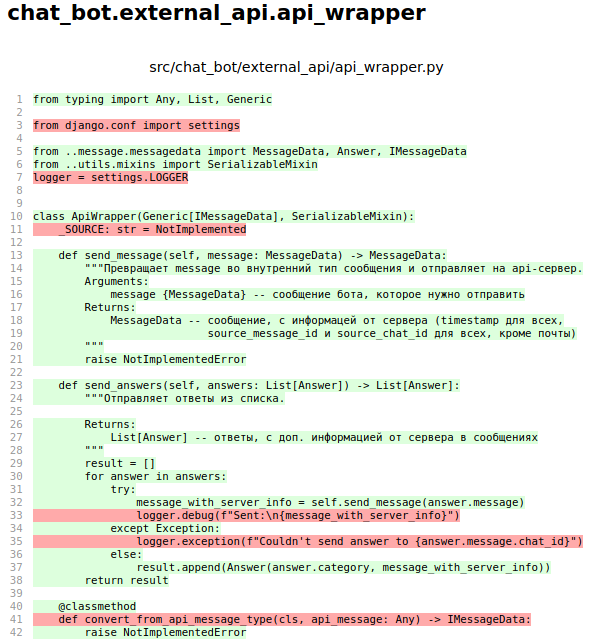
\includegraphics[width=\linewidth]{static/mypy-report.png}
        \caption{Отчет \textit{mypy} в формате html}
        \label{fig:mypy-report}
    \end{figure}
    
    \subsection{Автоматические тесты}
    Во время работы над проектом активно использовались модульные,
    интеграционные и системные тесты. \cite{test.kulikov}
    Для написания модульных тестов использовалась
    встроенная библиотека \textit{unittest} \cite{test.unittest}.
    Обязательными модульными тестами покрываются все публичные методы классов,
    приватные методы тестируются по мере их необходимости.
    Для интеграционных тестов,
    там где было необходимо проверить взаимодействие приложения с базой данных,
    использовалась библиотека \textit{django.test} фреймворка \textit{django}
    \cite{docs.django}.
    Для системных тестов, а именно проверки корректности работы веб-API
    приложения, использовалась библиотека \textit{tavern} \cite{test.tavern}.
    Сами тесты \textit{tavern} описываются в документе в формате yaml, при этом
    могут быть описаны адрес и содержимое запроса и
    проверены как код ответа сервера и его содержимое.
    Пример описания документа с тестом приведен на рисунке 17.
    \begin{figure}[H]
        \centering
        \lstinputlisting{snippets/tavern-test.yaml}
        \caption{Конфигурационный файл Tavern тестов}
        \label{fig:tavern-tests}
    \end{figure}

    Все тесты полностью автоматизированы, для этого использовался
    фреймворк \textit{pytest} \cite{test.pytest},
    предоставляющий библиотеку для написания тестов и
    утилиту для их запуска. Но в первую очередь фреймворк был выбран из-за его
    возможности объединять и совместно выполнять тесты
    \textit{unittest}, \textit{django.test} и \textit{tavern}.
    Всего в проекте зарегистрировано 209 модульных и интеграционных тестов и
    5 системных.

    \subsection{Нагрузочное тестирование}
    Нагрузочное тестирование проводилось на тестовом сервере на полностью
    развернутом веб-приложении с веб-сервером \textit{Nginx} при помощи
    инструмента Яндекс.Танк \cite{test.yandex.tank}.
    Целью нагрузочного тестирования было установление
    порога стабильной работы сервиса. Для этого на него подавалась нагрузка
    с константным количеством запросов в секунду в течение 2 минут с итеративным
    увеличением количества запросов.

    Конфигурационный файл для Яндекс.Танка на рисунке 18.
    \begin{figure}[H]
        \centering
        \lstinputlisting{snippets/load.yaml}
        \caption{Конфигурационный файл Яндекс.Танка}
        \label{fig:tank-load}
    \end{figure}

    Так, было установлено, что сервис стабильно выдерживает нагрузку до 20
    запросов в секунду в течение 2 минут.
    График, иллюстрирующий результаты тестирования, представлен на рисунке 19.
    \begin{figure}[H]
        \centering
        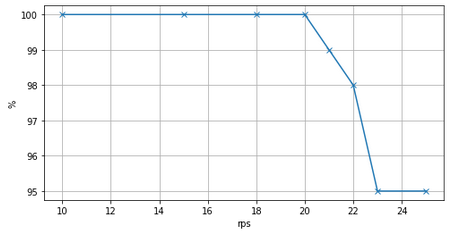
\includegraphics{static/tank-result.png}
        \caption{Результаты нагрузочного тестирования}
        \label{fig:tank-result}
    \end{figure}

    \subsection*{Вывод по главе 4}
    В этой главе мы рассмотрели виды тестирования, реализованные в новом проекте.
    В проекте были использованы модульные, интеграционные, системные и нагрузочные
    тесты для исследования и контроля за соответствием продуктом требуемых
    поведения и производительности,
    что в дальнейшем поможет в развитии и поддержке проекта.
